\documentclass[a4paper,10pt]{article}
%\documentclass[a4paper,10pt]{scrartcl}

\usepackage[utf8]{inputenc}

\usepackage{multirow}

\usepackage{graphicx}
  \graphicspath{ {../images/} }
  
\usepackage{color}
  \definecolor{lbcolor}{rgb}{0.9,0.9,0.9}
  \definecolor{lbkeywordcolor}{rgb}{0,0,0.89}
  \definecolor{lbcommentcolor}{rgb}{0.58,0.58,0.58}
  \definecolor{lbstringcolor}{rgb}{0.8,0.48,0}
  \definecolor{pathcolor}{rgb}{0.4,0.4,0.4}
  
  
\usepackage{listings}
\lstset{
  tabsize=4,
  basicstyle=\ttfamily,
  showstringspaces=false,
  backgroundcolor=\color{lbcolor},  
  keywordstyle=\color{lbkeywordcolor},
  commentstyle=\color{lbcommentcolor},
  stringstyle=\color{lbstringcolor},
  breaklines=true,
  xleftmargin=0.5cm,
  xrightmargin=0.5cm,
  framexleftmargin=0.25cm,
  framexrightmargin=0.25cm,
  %prebreak={\\}
}

%\lstdefinelanguage{bash} {
%  morekeywords={sudo,echo}
%}

\newcommand{\path}[1]{\textcolor{pathcolor}{\textbf{#1}}} %texttt

\usepackage{hyperref}
\hypersetup{
  colorlinks=true,
  linkcolor=black
}

\title{PointhiBoard Dokumentation}
\author{Thomas Pointhuber}
\date{}

\pdfinfo{
  /Title    (Pointhi Board Dokumentation)
  /Author   (Thomas Pointhuber)
  /Creator  (Thomas Pointhuber)
  /Producer ()
  /Subject  ()
  /Keywords (Raspberry Pi Shield)
}

\begin{document}
\maketitle

\pdfbookmark{\contentsname}{toc}

\tableofcontents


\newpage

\section{Einleitung}

Der Raspberry Pi ist ein einfacher Einplatinencomputer, welcher ideal für komplexe Steuerungs-/Regelungs- aufgaben im Bereich der Robotik, Hausautomatisierung, und vielen anderen Bereichen ist.\\
Er zeichnet sich durch einen niedrigen Stromverbrauch in Verbindung mit einer großen Anzahl von Schnittstellen, angefangen von USB und LAN über Bussysteme wie SPI und I2C bis zu einzelnen Digitalen Ausgängen, welche mithilfe von Linux angesprochen werden können.\\
Die Nutzung der Low-Level Schnittstellen die an einer Stiftleiste herausgeführt sind gestaltet sich aber nicht immer Trivial, auch ist die Spannungsversorgung in Robotern nicht für eine zusätzliche Last mit bis zu 1A ausgelegt. Aus diesem und anderen Gründen soll daher ein Erweiterungsboard für den Raspberry Pi entstehen welches grundlegende Aufgaben übernimmt, die für Systeme in Steuerungssystemen notwendig erscheinen.\\
%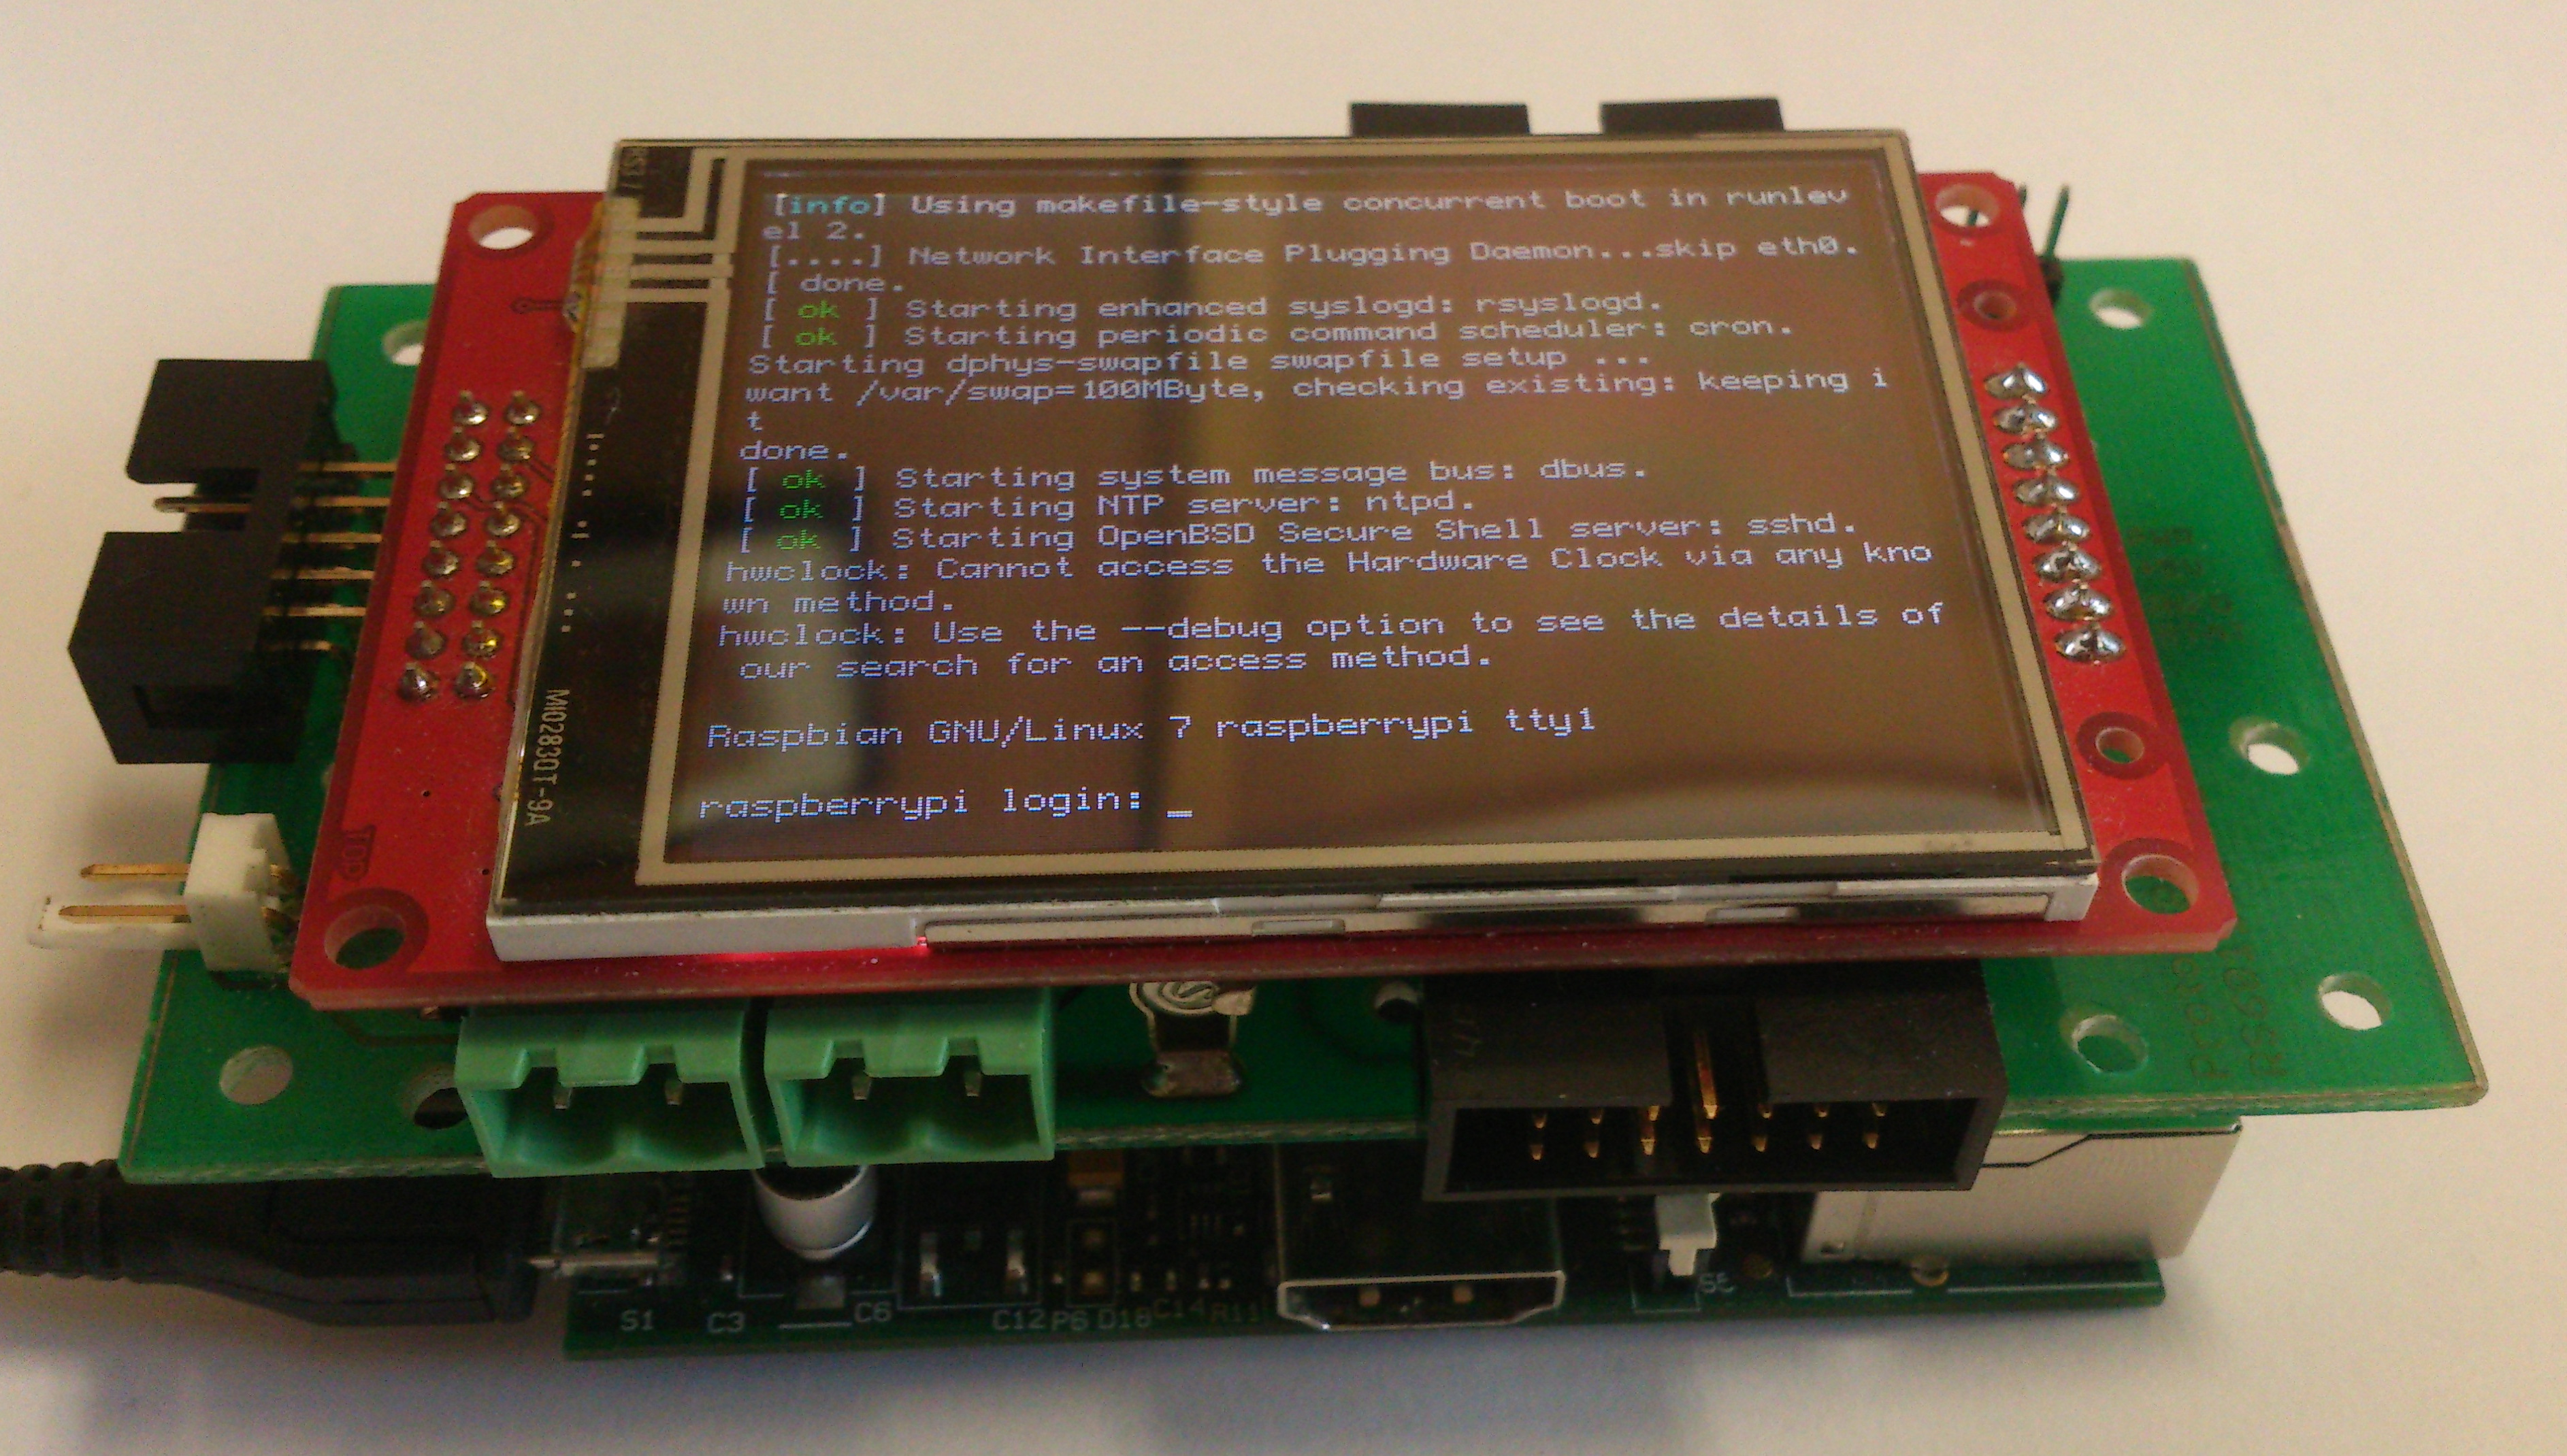
\includegraphics[width=\textwidth]{pointhiboard_booting}

\subsection{Überblick der Funktionen}
Die Grundlegenden Ausstattung, die die Erweiterungsplatine besitzen soll, bzw. bereits besitzt.
\begin{itemize}
 \item Effizienter Spannungsregler der Spannungen zwischen 7V-25V auf saubere 5V regelt
 \item Pegelwandler für I2C, um sich mit normaler 5V-Hardware  zu verbinden
 \item Schnittstelle für LCD-Touch-Display auf SPI-Basis, welche später auch für SPI$\rightarrow$CAN Konverter benutzt werden kann.
 \item Echtzeituhr (RTC), weil der Raspberry Pi keine besitzt, diese aber für diverse Anwendungen benötigt werden
 \item Spannungsüberwachung und Überstromschutz, um auch mit LiPo-Versorgung sicher zu arbeiten (Tiefentladeschutz)
 \item Digitale Ein/Ausgänge und 8 Analoge Eingänge um ohne zusätzlicher Erweiterungsboard bereits einfache Steuerungen zu realisieren.
 \item RS232-TTL Schnittstelle
 \item RN-Standard Steckverbinder mit Verriegelung, für einfache Erweiterbarkeit und Betriebssicherheit.
\end{itemize}

\section{Technische Spezifikationen}

\subsection{Mechanische Spezifikationen}

\begin{center}
    \begin{tabular}{| l | l | l | l | l |}
    \hline
    Characteristic & Min & Typ. & Max & Units \\ \hline
    Breite & - & 60 & - & mm \\ \hline
    Länge & - & 110 & - & mm \\ \hline
    
    \end{tabular}
\end{center}

\subsection{Elektrischer Spezifikationen}

\begin{center}
    \begin{tabular}{| l | l | l | l | l | l | l |}
    \hline
    Characteristic 	& Symbol 	& Test Conditions 	& Min 	& Typ. 	& Max 	& Units \\ \hline
    Versorgungsspannung & $U_{IN}$ 	& 			& 8 	& 12 	& 20 	& $V$ \\ \hline
    Eingangsstrom 	& $I_{IN}$ 	& 			& - 	& - 	& 8 	& $A$ \\ \hline
    Leerlaufstrom 	& $I_{IN0}$ 	& $U_{IN} = 12V$	& - 	& 20 	& - 	& $mA$ \\ \hline
    Ausgangsspannung, 5V& $U_{5V}$ 	& 			& 4.95 	& 5 	& 5.05 	& $V$ \\ \hline
    Ausgangsstrom, 5V 	& $I_{5V}$ 	& 			& - 	& - 	& 2.5 	& $A$ \\ \hline
    Umgebungstemperatur &  		& 			& -10 	& 20 	& 50 	& $^\circ C$ \\ \hline
    \end{tabular}
\end{center}

\subsubsection{Steckverbinder}

\paragraph{I2C} \mbox{} \\

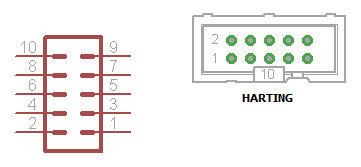
\includegraphics[scale=0.6]{connector_i2c} \\
Der I2C-Stecker ist gemäß den RN-Definitionen\footnote{\url{http://www.rn-wissen.de/index.php/RN-Definitionen\#I2C-Bus_Stecker}} belegt.
\begin{center}
    \begin{tabular}{| l | l |}
    \hline
    Pin 1 	& SCL (Taktleitung) \\ 
    Pin 3	& SDA (Datenleitung) \\
    Pin 5,7 	& +5V \\ 
    Pin 9 	& Batteriespannung \\ 
    Pin 2,4,6,8	& GND \\
    Pin 10 	& INT \\ \hline
    \end{tabular}
\end{center}

\paragraph{ICSP} \mbox{} \\

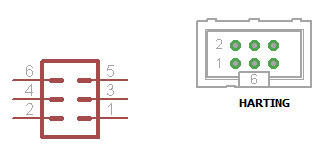
\includegraphics[scale=0.6]{connector_icsp} 
\begin{center}
    \begin{tabular}{| l | l |}
    \hline
    Pin 1 	& PGD \\ 
    Pin 2,4	& VSS (GND) \\
    Pin 3 	& PGC \\ 
    Pin 5 	& VDD (+5V) \\ 
    Pin 6	& MCLRE/VPP \\ \hline
    \end{tabular}
\end{center}

\paragraph{8-Bit} \mbox{} \\

%\footnote{\url{http://www.rn-wissen.de/index.php/RN-Definitionen\#Datenportstecker_10polig_.288_Ports.29}}

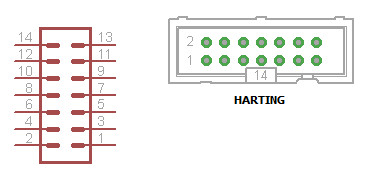
\includegraphics[scale=0.6]{connector_8-bit}
\begin{center}
    \begin{tabular}{| l | l |}
    \hline
    Pin 1...8 	& PIN 0...7 \\ 
    Pin 9,11	& +5V \\
    Pin 10,12,14& GND \\ 
    Pin 13 	& Batteriespannung \\ \hline
    \end{tabular}
\end{center}

\paragraph{RS232-TTL} \mbox{} \\


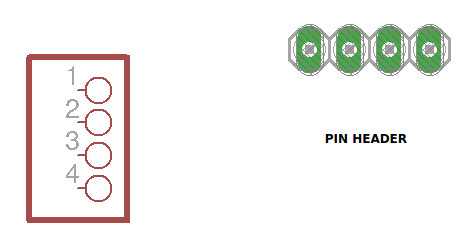
\includegraphics[scale=0.6]{connector_rs232-ttl} \\
Der RS232-TTL-Stecker ist gemäß den RN-Definitionen\footnote{\url{http://www.rn-wissen.de/index.php/RN-Definitionen\#RS232_TTL_Stecker}} belegt.
\begin{center}
    \begin{tabular}{| l | l |}
    \hline
    Pin 1 	& RX \\ 
    Pin 2	& TX \\
    Pin 3	& GND \\ 
    Pin 4 	& +5V \\ \hline
    \end{tabular}
\end{center}

%\section{Prototyp}

%Ich habe bereits einen Prototypen gebaut, der die grundlegende Funktionalität abdeckt, und als Testsystem dient. Das Linux-System bootet, und auch der Steuerungs-Chip auf dem Board arbeitet einwandfrei. Bis zu diesem Stand musste ich aber viele Probleme lösen, und deshalb wird bald eine neue Platine entstehen in der diese Probleme nicht mehr existent sind. \\ \\
%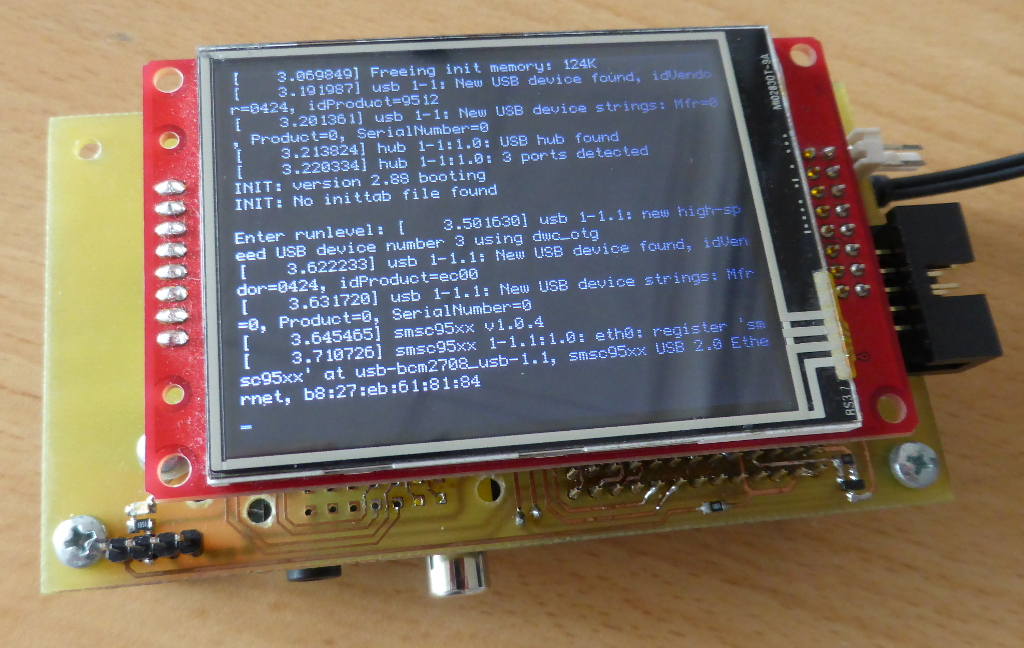
\includegraphics[width=\textwidth]{pointhiboard_prototype_booting} \\
%Das Board bekam bereits ein neues Layout, welches unter anderem Masseschleifen entfernte, und Status LEDs beinhaltet, die ein einfaches Debuggen ermöglichen sollen. Auch wurde der Schaltregler optimiert, welcher für das Board essentiell ist. \\

\section{Platine}

\subsection{Übersicht}

\subsubsection{Top-Layer}

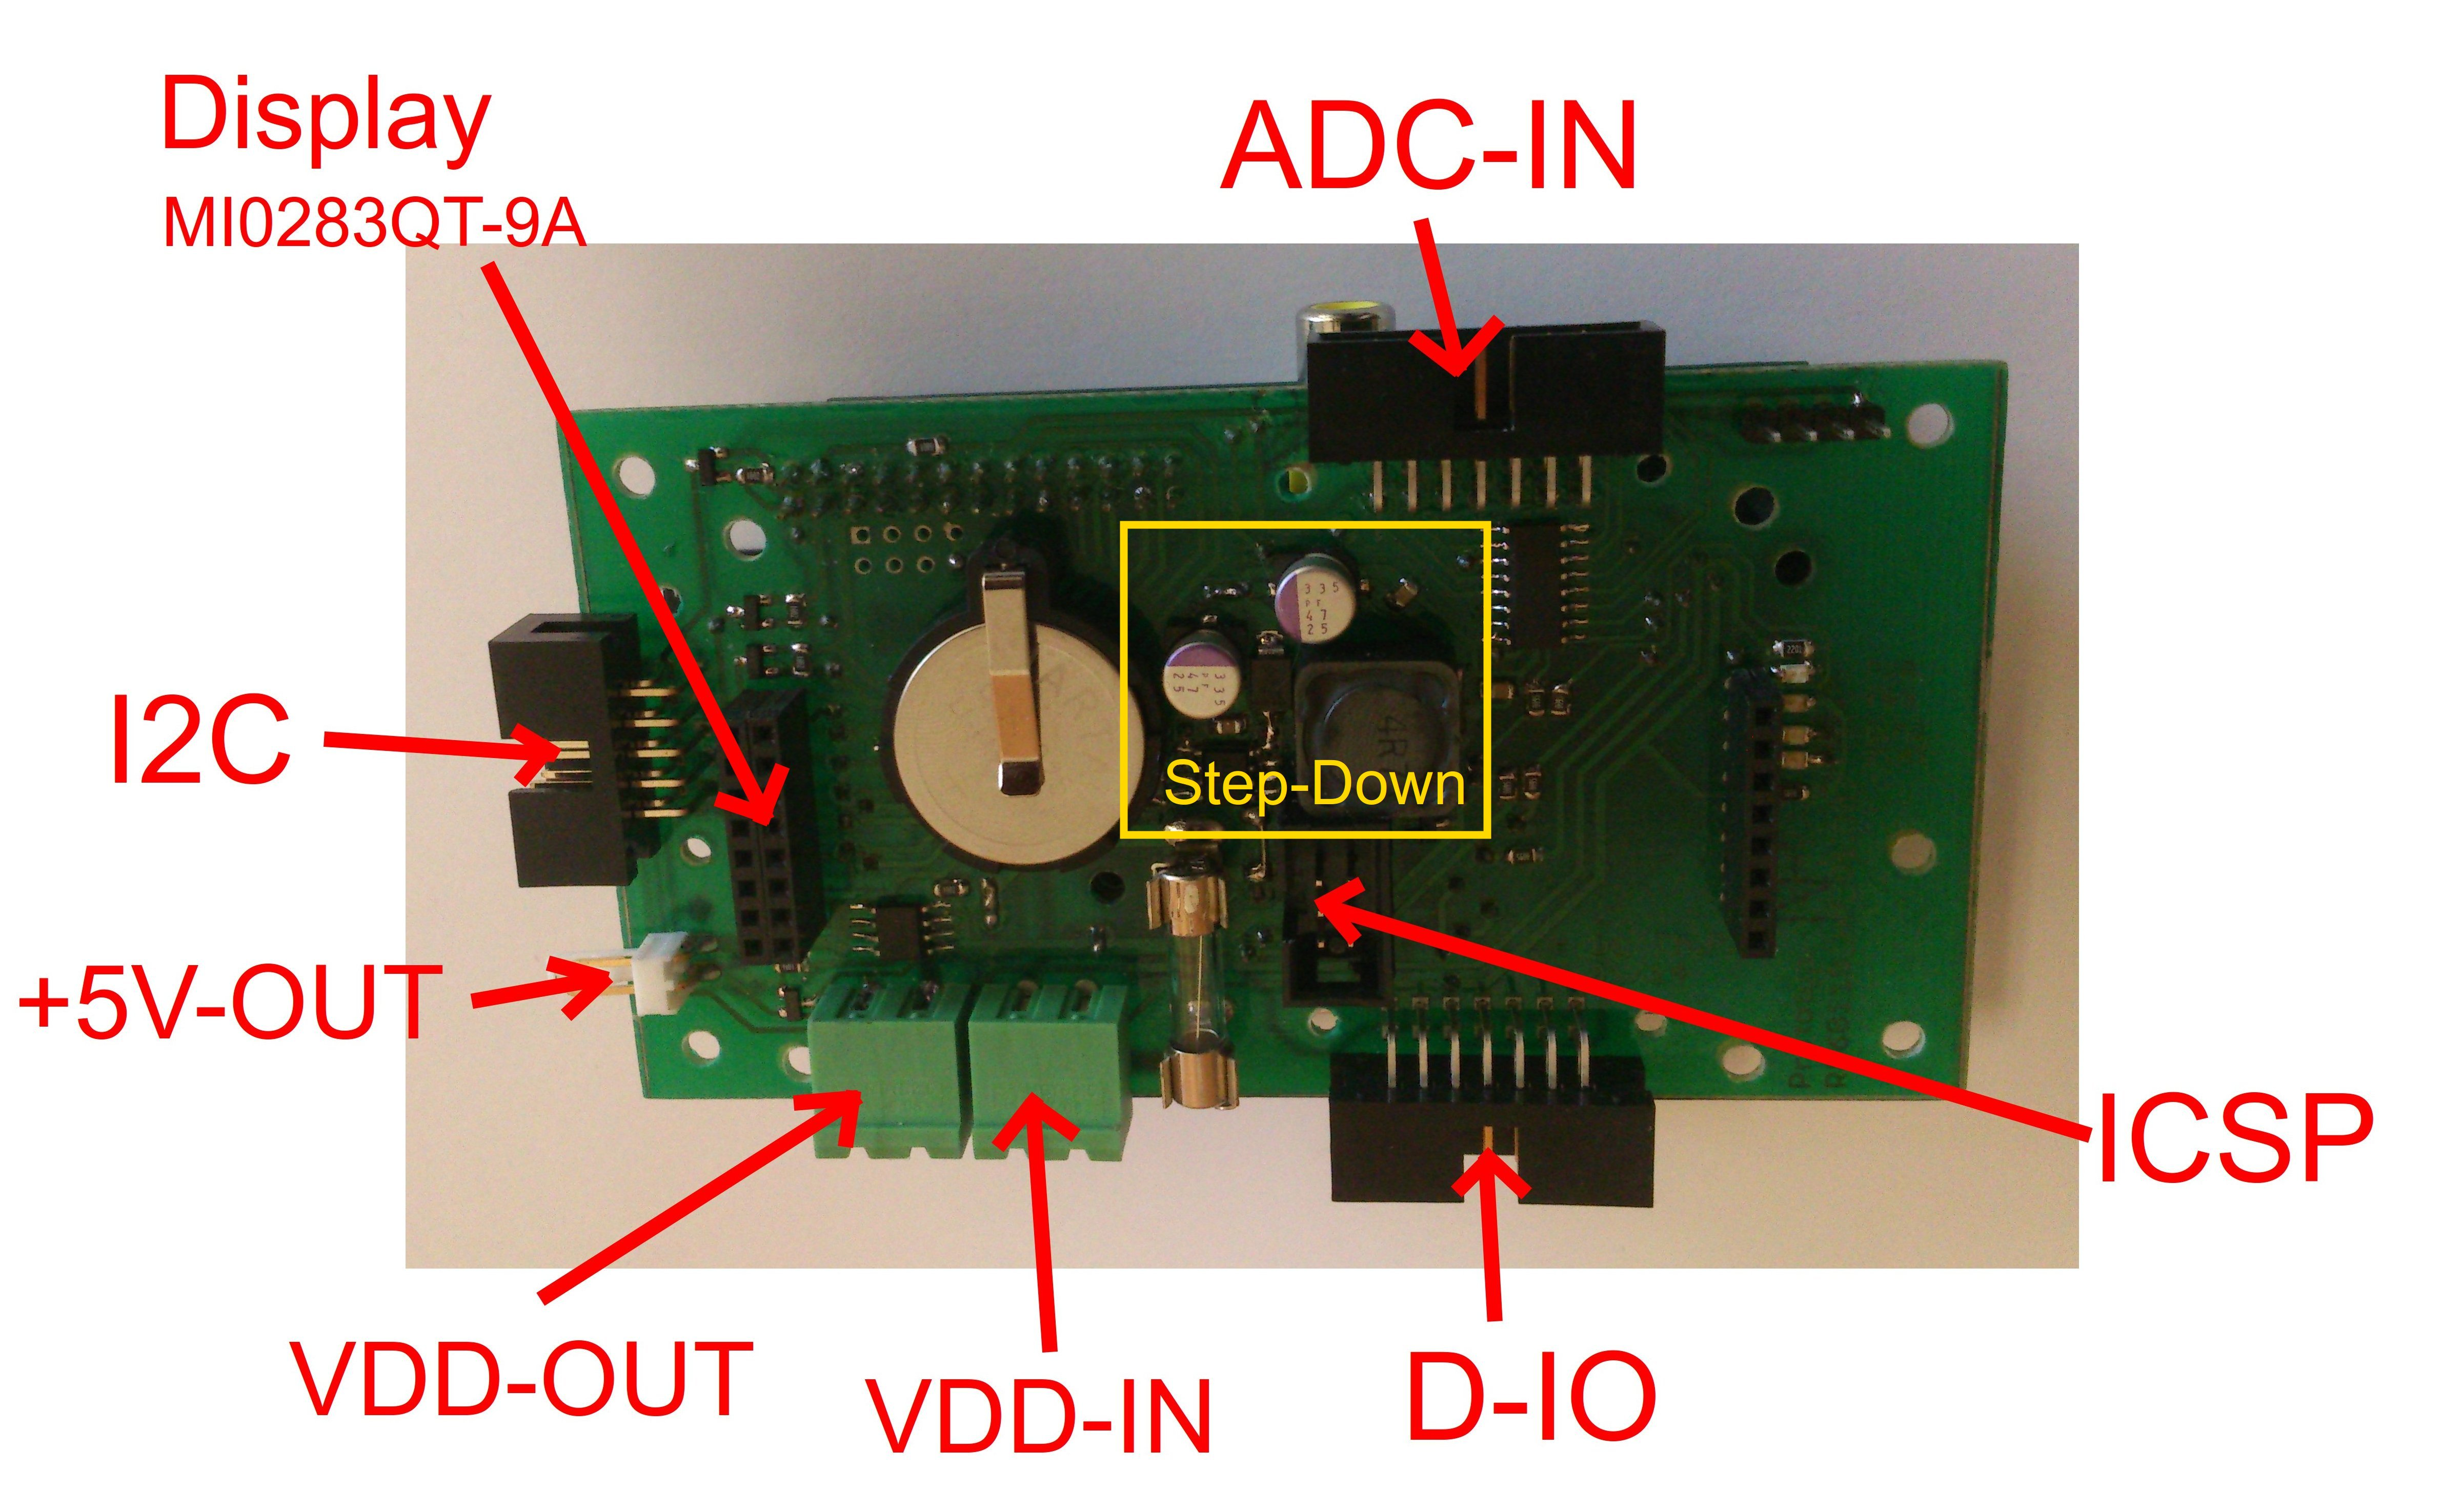
\includegraphics[width=\textwidth]{pointhiboard_overview_top}

\subsubsection{Bottom-Layer}

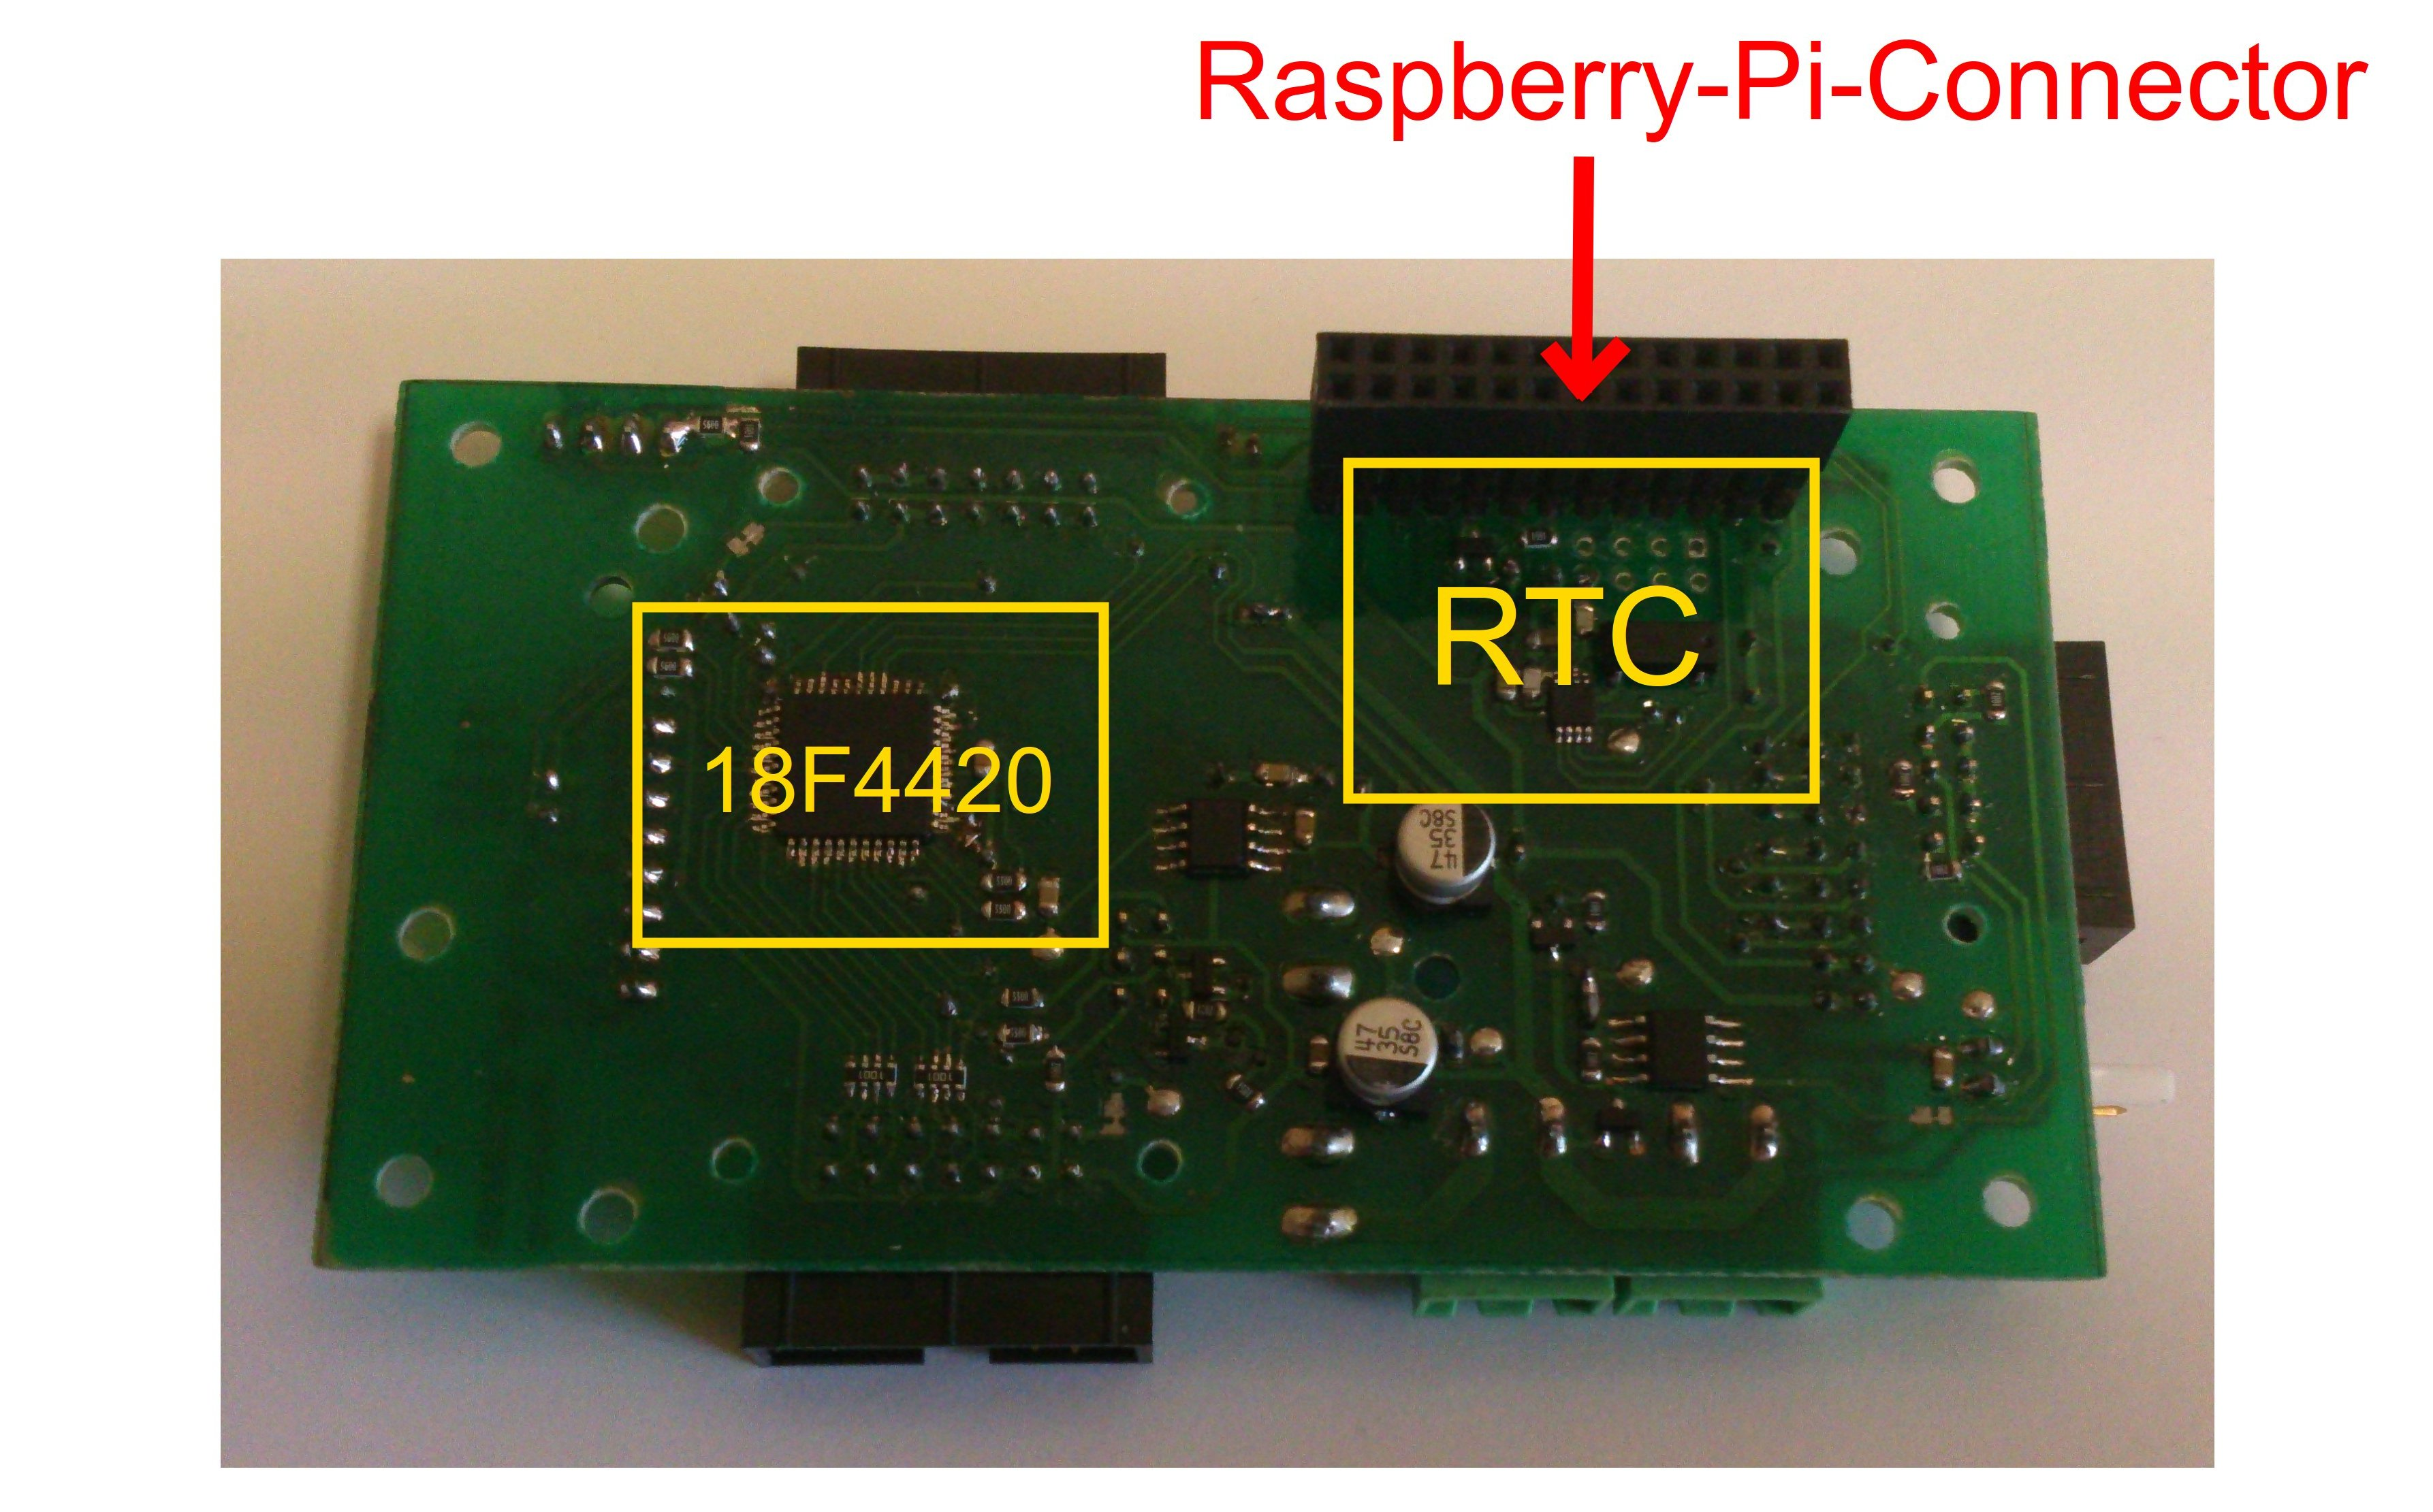
\includegraphics[width=\textwidth]{pointhiboard_overview_bottom}

\newpage
\subsection{Bestückung}

Es sollten zuerst alle SMD-Bauteile auf dem Bottom-Layer, danach die auf dem Top-Layer bestückt werden. Am Schluss werden noch alle Steckverbinder und die Batteriehalterung angelötet, wobei die große Buchsenleiste, die mit dem Raspberry Pi verbunden wird als letztes angelötet werden sollte. 

\subsubsection{Top-Layer}

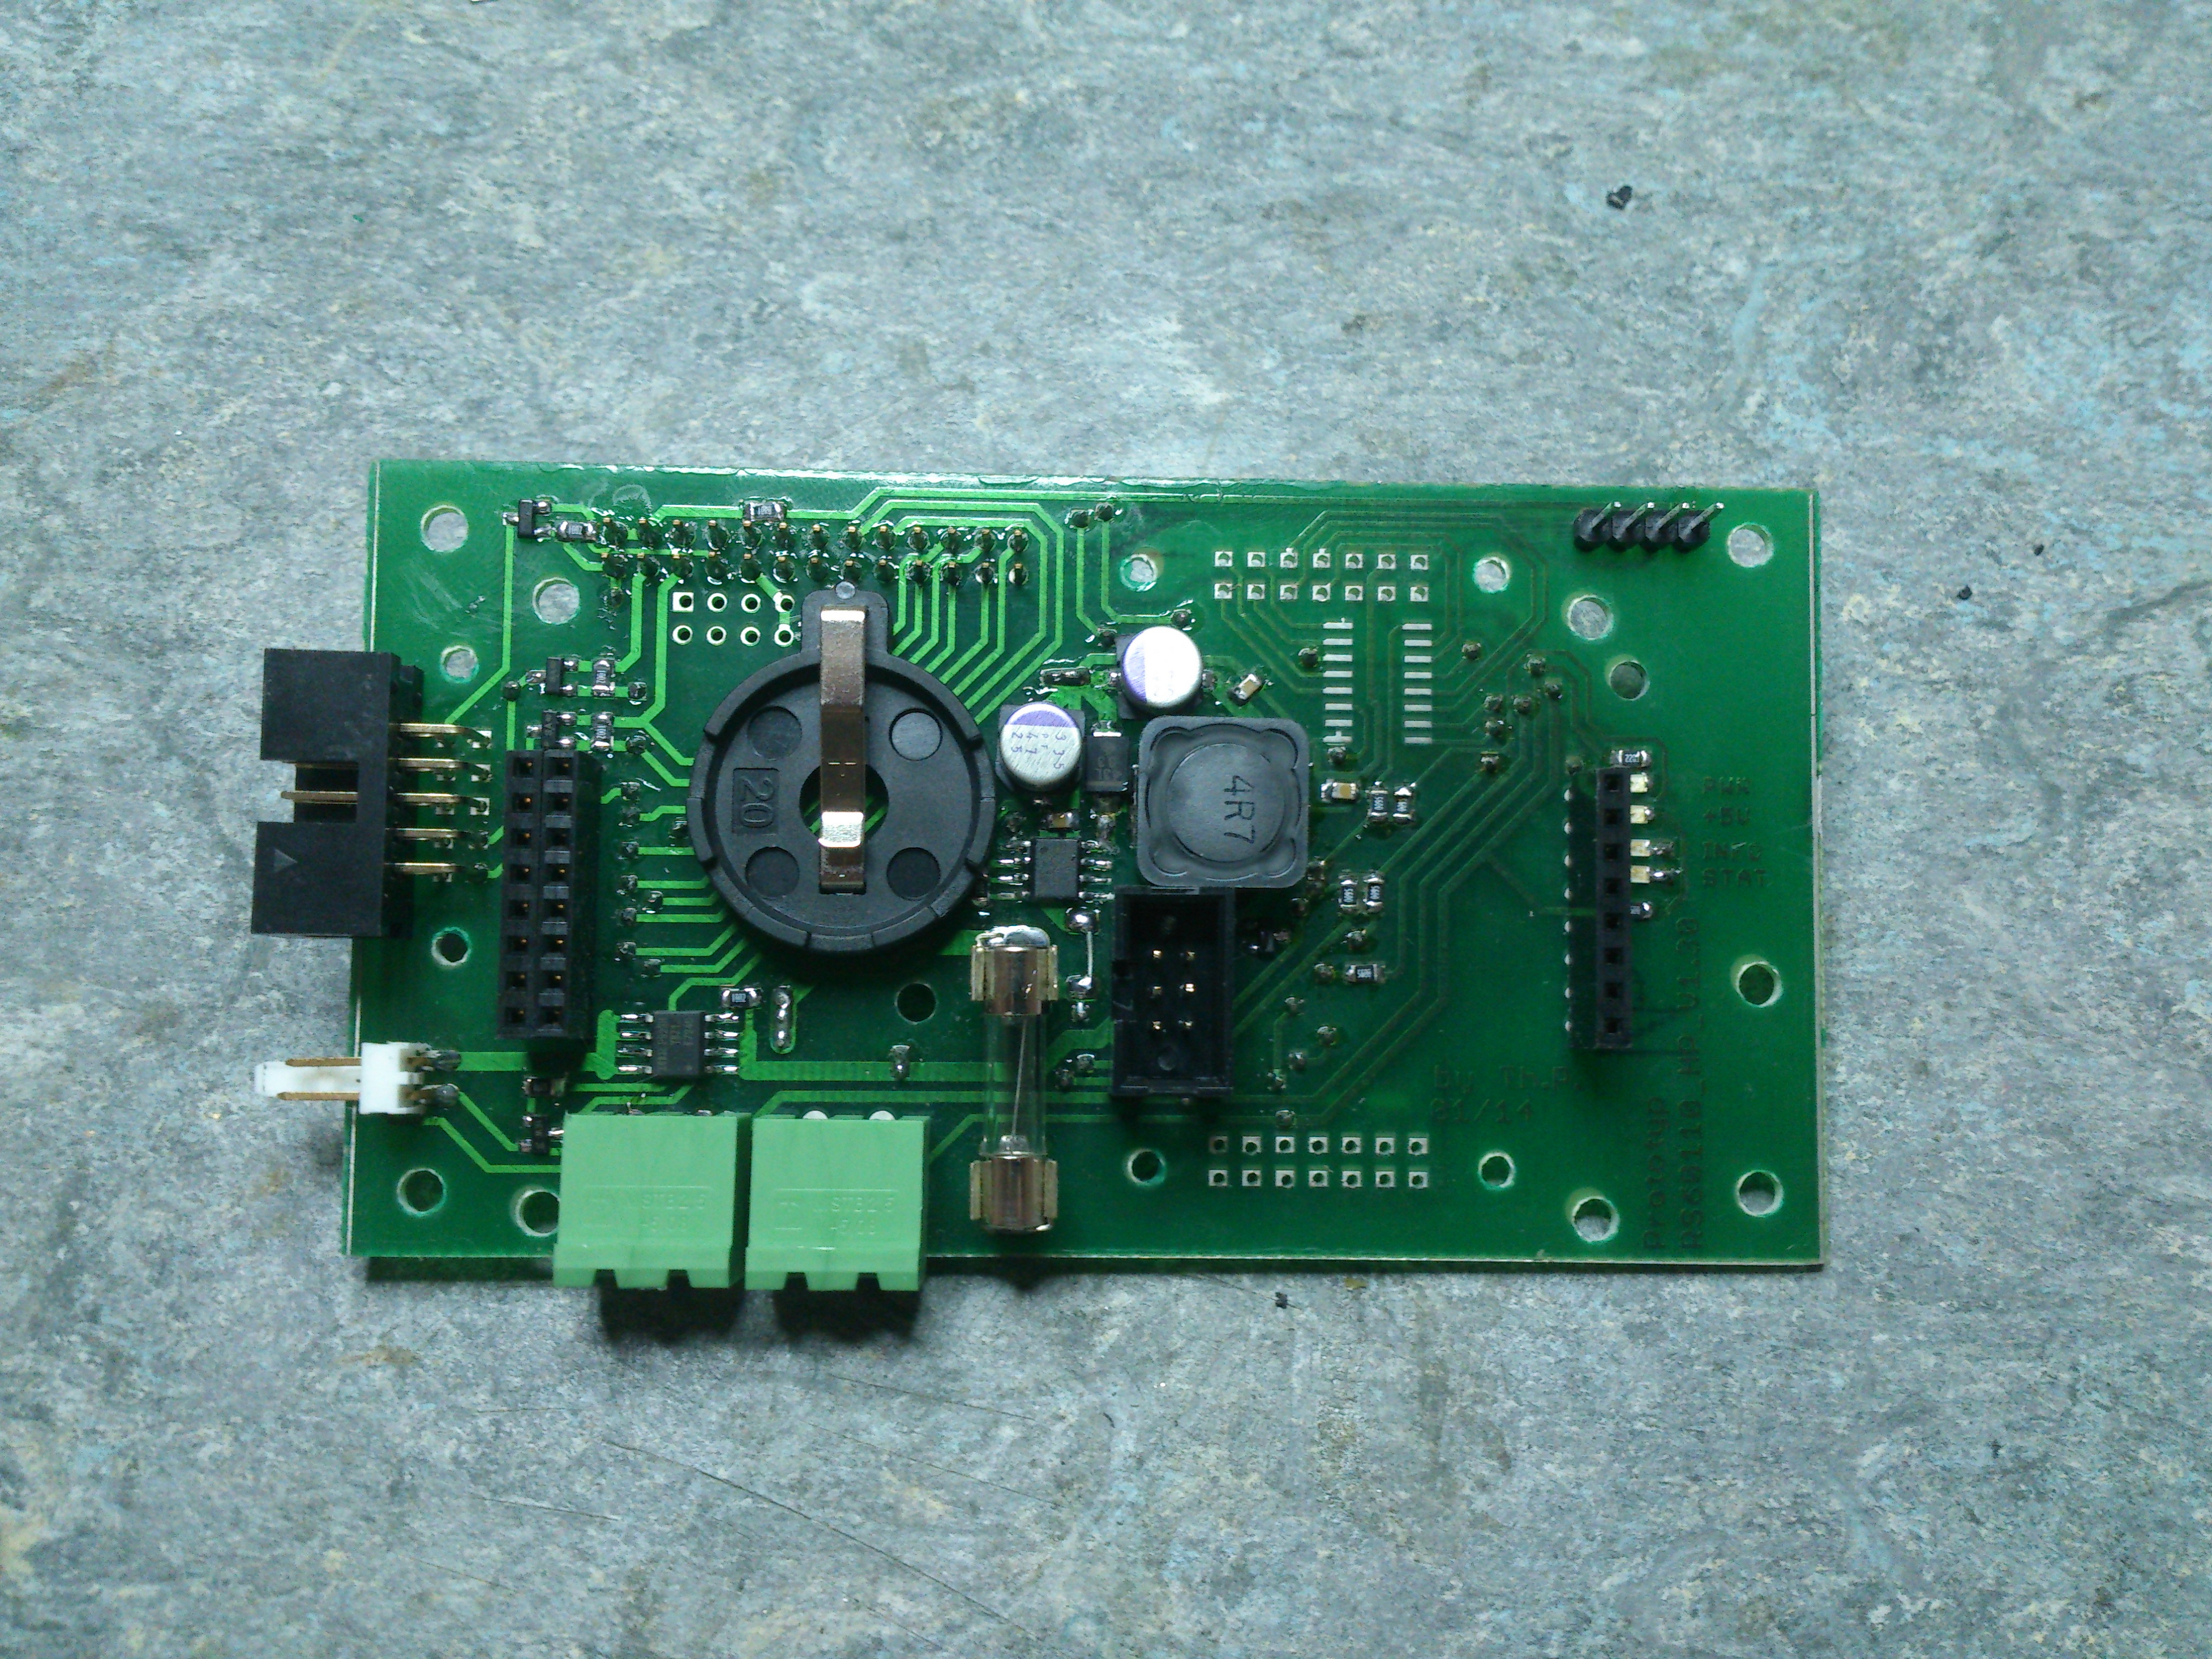
\includegraphics[width=\textwidth]{pointhiboard_board_top} \\

\subsubsection{Bottom-Layer}

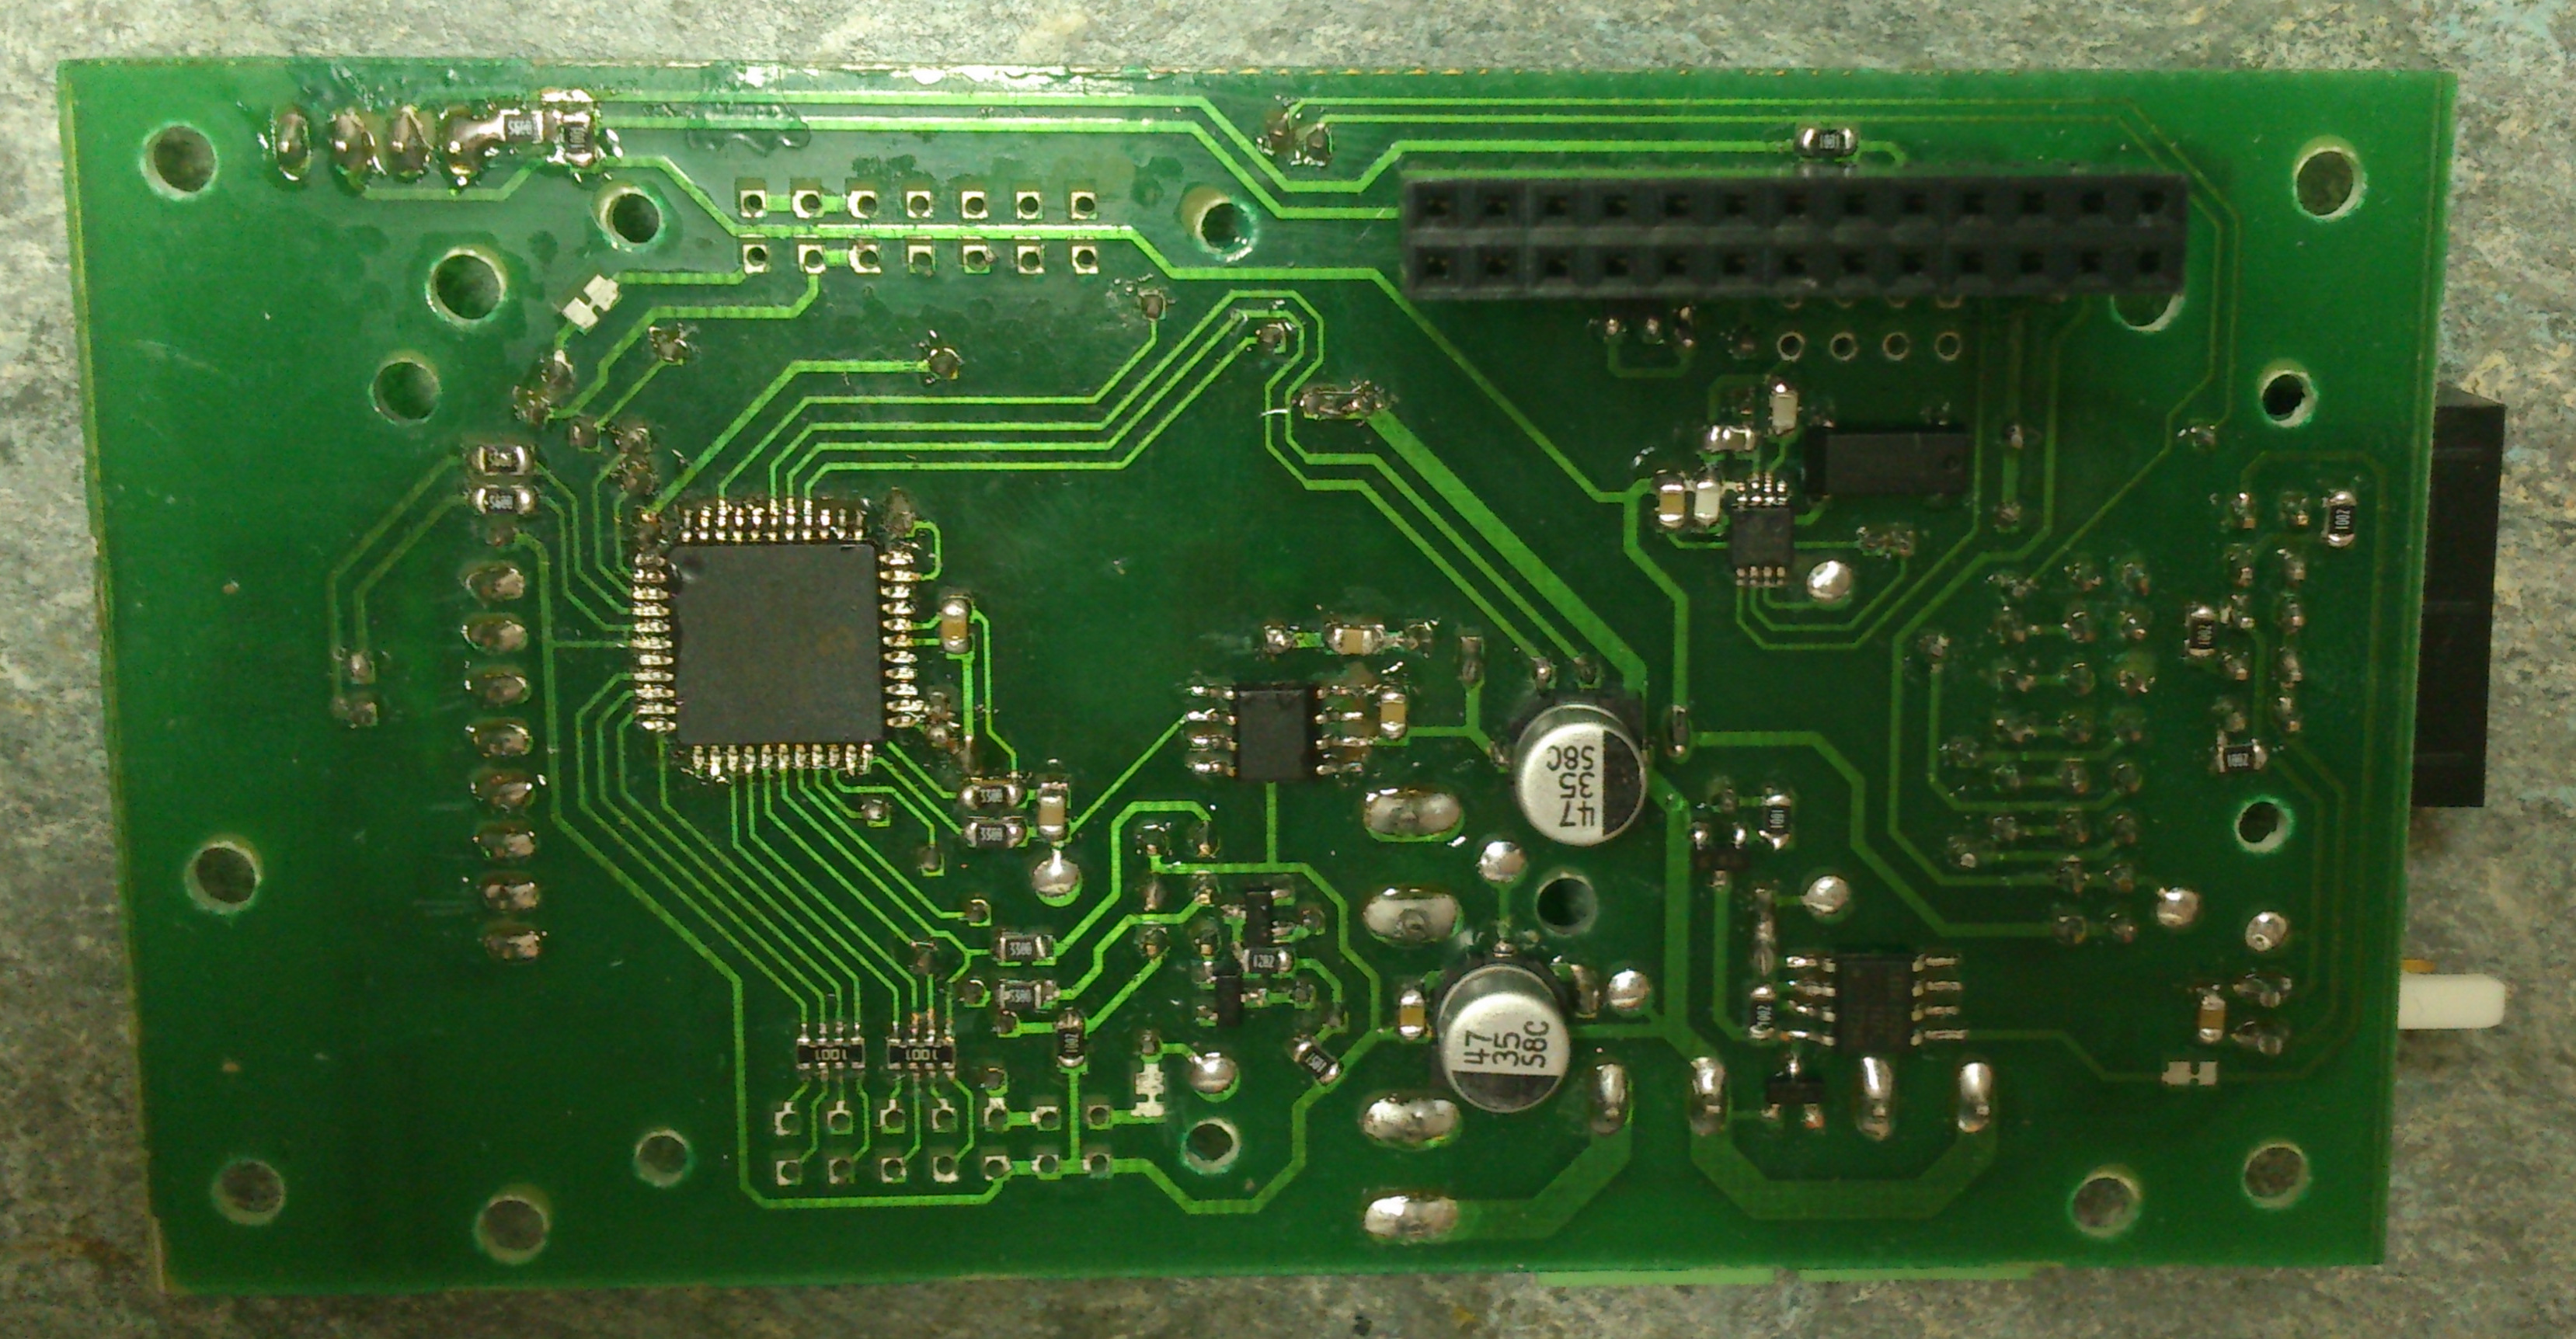
\includegraphics[width=\textwidth]{pointhiboard_board_bottom} \\

\newpage

\section{Inbetriebnahme der Hardware}

\subsection{Flashen des Steuer-PIC}

Es wird ein ICSP-Programmiergerät, welches einen PIC18F4420 flashen kann am Board angeschlossen (ICSP-Stecker). Der PIC sollte korrekt erkannt werden, und kann dann mit der Firmware beschrieben werden.

\subsection{Testen des Step-Down-Wandler}

\begin{enumerate}
 \item Es wird am Eingang des Board ein Netzteil mit folgenden Einstellungen angeschlossen: $I_{max} ~= 100mA, U_a = 5V$
 \item Am Spannungs-Ausgang für den Raspbery Pi wird ein Multimeter angeschlossen, welches eine Spannung von ungefähr 5V anzeigen sollte.
 \item Jetzt wird die Spannung des Netzteiles langsam auf etwa 10-12V gesteigert, die Spannung am Multimeter darf dabei eine Spannung von 5,1-5,2V nicht überschreiten!
Falls die Spannung höher als etwa 5,2V steigen sollte funktioniert der Step-Down-Wandler nicht ordnungsgemäß. Der Step-Down-Wandler auf der Platine muss überprüft und wenn möglich repariert werden. Eine zu hohe Spannung am 5V-Spannungskreis könnte ansonsten zu einer Beschädigung diverser Bauteile auf dieser, und anderen angeschlossenen Platinen führen.
\end{enumerate}

\subsection{Fehlerbehebung}

\begin{center}
    \begin{tabular}{| l | p{6cm} |}
    \hline
    Problem 							& Fehlerursache \\ \hline
    \multirow{3}{*}{Keine der Status-LED leuchtet auf}
	& Board nicht korrekt angeschlossen \\ \cline{2-2}
	& Sicherung durchgebrannt \\ \cline{2-2}
	& PIC nicht/falsch geflasht \\
    \hline
    \multirow{2}{*}{+5V, PWR-Led leuchtet nicht}
	& Tiefentladeschutz aktiv (kurz aufleuchtende STAT-LED) \\ \cline{2-2}
	& MOSFET schaltet nicht durch \\
    \hline
    \end{tabular}
\end{center}

\subsection{Testen der Hardware}

Der PIC wird mit der speziellen TEST-Firmware beschrieben\footnote{siehe Flashen des Steuer-PIC}. Dann werden die beiden 14-Poligen Stiftleisten 1:1 miteinander verbunden. Sobald das Board mit Spannung versorgt wird startet die Testroutine. Solange die Testroutine aktiv ist blinken beide Status-LEDs schnell. Wenn diese dann erfolgreich war, Leuchtet STAT dauerhaft. Falls die Testroutine fängt INFO zu blinken an.

\newpage

\section{Inbetriebnahme der Software}

Hier ist die Konfiguration einen Raspberry Pi der 2. Revision beschrieben. Wenn ein Raspberry Pi der 1. Revision verwendet wird muss i2c-1 durch i2c-0 ersetzt werden! Das verwendete Distribution ist das oft verwende Wheezy, bei Arch und anderen Linux Derivaten kann die Konfiguration abweichen!

\subsection{Aktivieren von I2C und SPI}

\begin{enumerate}
 \item In der Datei \path{/etc/modprobe.d/raspi-blacklist.conf} werden die beiden Schnittstellen aktiviert, indem die beiden Zeilen wie folgt auskommentiert werden:
    \begin{lstlisting}
#blacklist spi-bcm2708
#blacklist i2c-bcm2708
    \end{lstlisting}
 \item In der Datei \path{/etc/modules} werden dann folgende Module hinzugefügt:
    \begin{lstlisting}
snd-bcm2835
i2c-bcm2708 
i2c-dev     
    \end{lstlisting}
\end{enumerate}

\subsection{Aktivieren der I2C-Echtzeituhr}
\let\thefootnote\relax\footnote{\url{http://www.100randomtasks.com/raspberry-pi-rtc}}

\begin{enumerate}
 \item Hinzufügen der folgenden Zeile in der Datei \path{/etc/modules}:
    \begin{lstlisting}
i2c:mcp7941x
    \end{lstlisting}
 \item Es werden 2. Zeilen in der Datei \path{/etc/rc.local} hinzugefügt (vor dem Befehl ``exit 0``):
    \begin{lstlisting}[language=sh]
echo mcp7941x 0x6f > /sys/class/i2c-dev/i2c-1/device/new_device 
hwclock -s
    \end{lstlisting}
 \item Jetzt kann man die fake-hwclock deaktivieren
    \begin{lstlisting}[language=sh]
sudo update-rc.d fake-hwclock remove
    \end{lstlisting}
 \item Jetzt wird der Raspberry Pi neu gestartet, und dann die aktuelle zeit wie folgt in UTC gesetzt (natürlich das Datum durch das aktuelle ersetzten): 
    \begin{lstlisting}[language=sh]
sudo date -s "9 JAN 2014 12:00:00"
    \end{lstlisting}
 \item Beim Herunterfahren wird dann ab sofort die Zeit in die Echtzeituhr geschrieben, und beim nächsten Starten daraus ausgelesen.
\end{enumerate}

\subsubsection{Fehlerbehebung}

Falls wie bei mir die folgende Fehlermeldung hwclock: ''ioctl(RTC\_RD\_TIMEE) to /dev/rtc0 to read the time failed: Invalid argument`` auftritt, werden einfach die folgenden Befehle in die Shell der Reihe nach eingegeben:
\begin{lstlisting}[language=sh]
hwclock -w
hwclock -s
hwclock -r
\end{lstlisting}

\subsection{Aktivieren des LCD-Touch-Displays (MI0283QT-9A)}
\let\thefootnote\relax\footnotetext{\url{http://lallafa.de/blog/2013/07/watterotts-new-rpi-shieldbridge}}
\let\thefootnote\relax\footnotetext{\url{http://busware.de/tiki-index.php?page=CCD_Installation}}
\let\thefootnote\relax\footnotetext{\url{http://www.raspberrypirobot.com/1-8-tft-lcd-display-raspberry-pi-expansion-board/}}

\begin{enumerate}
 \item Download ''FBTFT drivers as loadable modules. See 'Step-by-step' for loading drivers.'' \url{https://github.com/notro/fbtft/wiki#image-download}
 \item In der Datei \path{/etc/modules} werden dann folgende Module hinzugefügt:
    \begin{lstlisting}
fbtft_device
ads7846_device
    \end{lstlisting}
 \item In der Datei \path{/etc/modprobe.d/pointhiboard.conf} werden dann folgende Optionen definiert:
    \begin{lstlisting}
options ads7846_device cs=0 speed=2000000 model=7846 x_min=250 x_max=3780 y_min=160 y_max=3930 pressure_max=255 x_plate_ohms=60 gpio_pendown=25 keep_vref_on=1 swap_xy=1 
options fbtft_device cs=1  speed=16000000 fps=25 name=mi0283qt-9a gpios=reset:23,led:24 rotate=90
    \end{lstlisting}
 \item In der Datei \path{/etc/X11/xinit/xinitrc} wird dann folgendes vor . /etc/X11/Xsession eingefügt:
    \begin{lstlisting}[language=sh]
# Touchpanel: Invert X and Y axis
DISPLAY=:0 xinput --set-prop 'ADS7846 Touchscreen' 'Evdev Axis Inversion' 1 1
    \end{lstlisting}
 \item Damit die Konsole beim booten auf dem Display dargestellt wird, muss folgendes am ende in \path{/boot/cmdline.txt} hinzugefügt werden:
    \begin{lstlisting}
fbcon=map:10 fbcon=font:ProFont6x11
    \end{lstlisting}
\end{enumerate}

\newpage

\section{PIC-Firmware}

\subsection{I2C}

\subsubsection{Schreiben}

Das erste übertragene Byte setzt den Schreib/Lese-Index fest. Dieser wird dann nach jedem weiteren Schreib/Lesebefehl jeweils um 1 inkrementiert, solange er nicht neu gesetzt wurde.

\begin{center}
    \begin{tabular}{| l | l | l |}
    \hline
    Index 	& Aktion 	& Information \\ \hline
    0x01 	& Setze TRISB 	& 1... Eingang, 0... Ausgang \\ \hline
    0x0F 	& Setze PORTB 	& 1... High, 0... Low \\ \hline
    \end{tabular}
\end{center}

\subsubsection{Lesen}

\begin{center}
    \begin{tabular}{| l | l | l |}
    \hline
    Index 	& Aktion 			& Information \\ \hline
    0x01 	& Lese TRISB 			& 1... Eingang, 0... Ausgang \\ \hline
    0x0F 	& Lese PORTB 			& 1... High, 0... Low \\ \hline
    0x10 	& ADC - 0 VOLTAGE-HIGH-BYTE 	& \\ \hline
    0x11 	& ADC - 0 VOLTAGE-LOW-BYTE 	& \\ \hline
    0x12 	& ADC - 1 VOLTAGE-HIGH-BYTE 	& \\ \hline
    0x13 	& ADC - 1 VOLTAGE-LOW-BYTE 	& \\ \hline
    0x14 	& ADC - 2 VOLTAGE-HIGH-BYTE 	& \\ \hline
    0x15 	& ADC - 2 VOLTAGE-LOW-BYTE 	& \\ \hline
    0x16 	& ADC - 3 VOLTAGE-HIGH-BYTE 	& \\ \hline
    0x17 	& ADC - 3 VOLTAGE-LOW-BYTE 	& \\ \hline
    0x18 	& ADC - 4 VOLTAGE-HIGH-BYTE 	& \\ \hline
    0x19 	& ADC - 4 VOLTAGE-LOW-BYTE 	& \\ \hline
    0x1A 	& ADC - 5 VOLTAGE-HIGH-BYTE 	& \\ \hline
    0x1B 	& ADC - 5 VOLTAGE-LOW-BYTE 	& \\ \hline
    0x1C 	& ADC - 6 VOLTAGE-HIGH-BYTE 	& \\ \hline
    0x1D 	& ADC - 6 VOLTAGE-LOW-BYTE 	& \\ \hline
    0x1E 	& ADC - 7 VOLTAGE-HIGH-BYTE 	& \\ \hline
    0x1F 	& ADC - 7 VOLTAGE-LOW-BYTE 	& \\ \hline
    0x20 	& ADC - VCC VOLTAGE-HIGH-BYTE 	& \\ \hline
    0x21 	& ADC - VCC VOLTAGE-LOW-BYTE 	& \\ \hline
    0x22 	& ADC - +5V VOLTAGE-HIGH-BYTE 	& \\ \hline
    0x23 	& ADC - +5V VOLTAGE-LOW-BYTE 	& \\ \hline
    \end{tabular}
\end{center}

\end{document}
